\begin{frame}
    \frametitle{Course Objectives}

    \begin{itemize}
        \item Understand the fundamentals of Apache Spark.
        \item Build data processing applications using Apache Spark.
        \item Understand Apache Spark APIs (RDD, DataFrames, and Datasets).
        \item Optimize and tune Apache Spark applications.
        \item Build streaming applications using Apache Spark.
        \item Build scalable machine learning applications using Apache Spark MLlib.
        \item Deploy Apache Spark in production environments.
    \end{itemize}

\end{frame}

%%%%%%%%%%%%%%%%%%%%%%%%%%%%%%%%%%%%%%%%%%%%%%%%%%%%%%

\subsection{Course References}\label{subsec:course-references}
\begin{frame}
    \frametitle{\subsecname}
    \begin{itemize}
        \item \href{https://pages.databricks.com/rs/094-YMS-629/images/LearningSpark2.0.pdf}{Learning Spark, 2nd Edition} By Jules S. Damji, Brooke Wenig, Tathagata Das, Denny Lee.
        \item \href{https://learning.oreilly.com/library/view/spark-the-definitive/9781491912201/}{Spark: The Definitive Guide} By Bill Chambers, Matei Zaharia.
        \item Random blog posts.
    \end{itemize}
\end{frame}
%%%%%%%%%%%%%%%%%%%%%%%%%%%%%%%%%%%%%%%%%%%%%%%%%%%%%%

\subsection{Course Prerequisites}\label{subsec:course-prerequisites}
\begin{frame}
    \frametitle{\subsecname}
    Before beginning this course, participants should have:
    \begin{itemize}
        \item Experience in programming using Python.
        \item Basic programming skills using shell.
        \item An understanding of MapReduce foundations and Hive. \href{https://www.youtube.com/playlist?list=PLxNoJq6k39G8Ak39PDC-oYvp6ZRvIn3Pa}{Garage Education YouTube Playlist}
    \end{itemize}

\end{frame}

%%%%%%%%%%%%%%%%%%%%%%%%%%%%%%%%%%%%%%%%%%%%%%%%%%%%%%

% Ch.04-02   | Python Vs. Scala

\subsection{Python vs Scala}\label{subsec:python-vs-scala}
\begin{frame}
    \frametitle{\subsecname}
    \begin{itemize}
        \item Python is widely used with numerous tools and libraries available.
        \item Python is easier to learn than Scala; however, Scala might be more intuitive for those who prefer functional programming.
        \item Finding Python developers is generally easier for companies than finding Scala developers.
        \item Initially, Scala offered better performance in Apache Spark, but over time this advantage reduced, and now there's no big difference in speed.
        \item PySpark and Scala share the same Spark concepts, allowing for interchangeable use of examples from both languages without affecting learning.
    \end{itemize}
\end{frame}

\begin{frame}
    \begin{center}
        \begin{tcolorbox}[colback=blue!5!white,colframe=blue!75!black,title=Attention!]
            To Be a Spark Expert You Have to Be Able to Read a Little Scala Anyway!\footnote{Referenced from High Performance Spark, 2nd Edition, Ch.01}
        \end{tcolorbox}
    \end{center}

\end{frame}

%
\begin{frame}
    \frametitle{Spark's Codebase and Documentation}
    \begin{itemize}
        \item The quality of Spark's documentation is inconsistent.\footnote{Referenced from High Performance Spark, 2nd Edition, Ch.01}
        \item Spark's codebase is very readable.
        \item Understanding the Spark codebase benefits \textbf{advanced users}.
    \end{itemize}

\end{frame}

\begin{frame}
    \frametitle{Understanding Spark Through Scala}
    \begin{itemize}
        \item Scala helps you understand Spark deeply.\footnote{Referenced from High Performance Spark, 2nd Edition, Ch.01}
        \item Spark is written in Scala.
        \item To work with Spark's source code effectively, it's essential to understand (read) Scala.
    \end{itemize}

\end{frame}

\begin{frame}
    \frametitle{RDD and Scala's Influence}
    \begin{itemize}
        \item Scala's influence is evident in Spark's Resilient Distributed Datasets (RDD).\footnote{Referenced from High Performance Spark, 2nd Edition, Ch.01}
        \item RDD methods are similar to Scala's collection tools.
        \item Functions like map, filter, and reduce are similar in both.
        \item Knowing Scala makes it easier to understand how RDDs work.
    \end{itemize}

\end{frame}

\begin{frame}
    \frametitle{Spark as a Functional Framework}
    \begin{itemize}
        \item Spark uses functional programming principles.
        \item Concepts like immutability and lambda are key.
        \item Understanding functional programming helps in using Spark well.\footnote{Referenced from High Performance Spark, 2nd Edition, Ch.01}
    \end{itemize}

\end{frame}

%%%%%%%%%%%%%%%%%%%%%%%%%%%%%%%%%%%%%%%%%%%%%%%%%%%%%%


%%%%%%%%%%%%%%%%%%%%%%%%%%%%%%%%%%%%%%%%%%%%%%%%%%%%%%
% Ch.04-03   | Introduction

\subsection{Introduction to Apache Spark}\label{subsec:history-of-apache-spark}
\begin{frame}
    \frametitle{\subsecname}
    \begin{itemize}
        \item Apache Spark was initiated at UC Berkeley in 2009, leading to the publication of \href{https://www1.icsi.berkeley.edu/pubs/networking/ICSI_sparkclustercomputing10.pdf}{Spark: Cluster Computing with Working Sets} in 2010 by Matei Zaharia et al.
%    \item It aimed to address the limitations of Hadoop MapReduce, especially for iterative machine learning algorithms requiring multiple data passes.
        \item Spark was developed to improve processing efficiency over Hadoop MapReduce, which struggled with iterative tasks because it launched separate jobs and reloaded data for each one. This was particularly important for machine learning algorithms that need multiple data passes.
        \item Initially, Spark was designed for batch applications, but it quickly expanded to include streaming, SQL analytics, graph processing, and machine learning.
    \end{itemize}
\end{frame}
\begin{frame}
    \frametitle{\subsecname}
    \begin{itemize}
        \item By 2013, the project had more than 100 contributors, and now it has over 2,000 contributors with more than 39,000 commits. It has been donated to the Apache Software Foundation, guaranteeing its future as a vendor-independent project.
        \item Key milestones in its development are Spark 1.0 in 2014, Spark 2.0 in 2016, and Spark 3.0 in 2020, highlighting its evolution and broad acceptance.
    \end{itemize}
\end{frame}
\begin{frame}
    \frametitle{\subsecname}
    \begin{itemize}
        \item Apache Spark is a \textbf{unified engine} designed for large-scale distributed data processing, either on-premises in data centers or in the cloud.
        \item Spark provides \textbf{in-memory} storage for intermediate computations, making it much faster than Hadoop MapReduce.
        \item Spark offers rich, composable APIs, for example:
        \begin{itemize}
            \item Spark SQL: SQL for interactive queries.
            \item MLlib: for machine learning over big data and complex computations.
            \item Structured Streaming: for stream processing with near real-time data.
            \item GraphX: for graph processing.
        \end{itemize}
        \item \textbf{Optimized Execution Engine}: Spark's Catalyst optimizer and \texttt{Tungsten execution engine} optimize execution plans and generate efficient code for execution.
    \end{itemize}
\end{frame}

%Ch.04-04   | About Databricks

\subsection{About Databricks}\label{subsec:about-databricks}
\begin{frame}
    \frametitle{About Databricks}
    \begin{itemize}
        \item Databricks, founded by the early AMPlab team, joined the community to further develop Spark.
        \item The organization was founded to deliver a comprehensive analytics platform, streamlining Spark's application in big data processing and analytics.
        \item Databricks has bridged the gap between academic research and enterprise applications through its managed cloud service and significant contributions to the Spark project.
    \end{itemize}
\end{frame}
\begin{frame}
    \frametitle{Beyond Apache Spark}
    \begin{minipage}{\textwidth}
        \begin{tikzpicture}
            % Place image at the left side
            \node[anchor=west] (image) at (0,0) {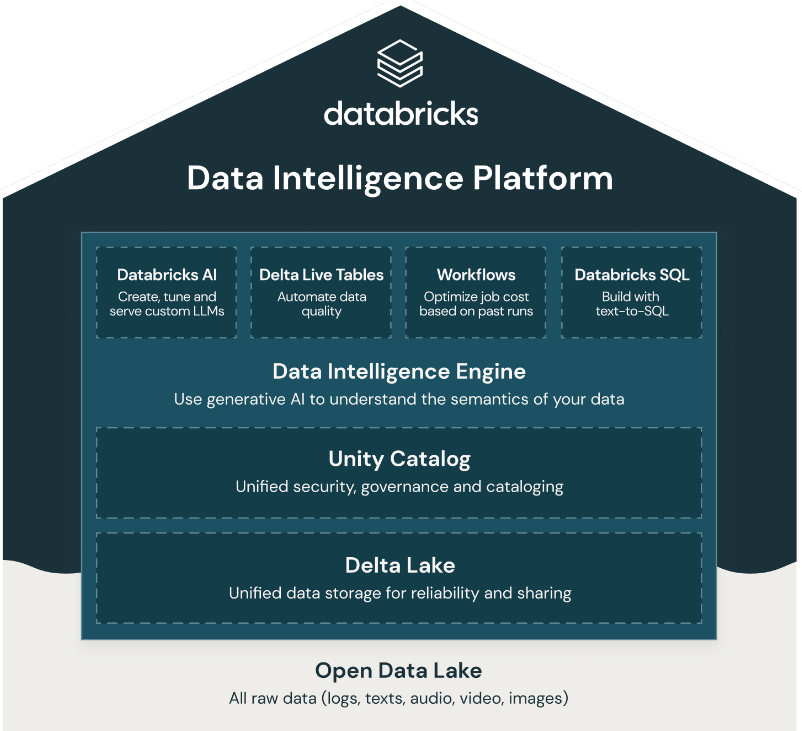
\includegraphics[width=\textwidth,height=.75\textheight,keepaspectratio]{./Figures/chapter-04/databricks_data_intelligence}};
            % Place text and arrow
            \draw[<-, thick] (image) -- ++(4,1) node[right, align=left,font=\small, text=gray] {Photo copied from\\ \url{https://www.datanami.com}};
        \end{tikzpicture}
        \captionof{figure}{Databricks Analytics Platform}
    \end{minipage}
\end{frame}

\begin{frame}
    \centering
    \vfill
    \Large{Do You Need Databricks to Work with Spark?}
    \vspace{1em}
    \vfill
\end{frame}

\begin{frame}
    \centering
    \vfill
    \Large{Do You Need Databricks to Work with Spark?}
    \hspace{1cm}
    \Large{\textcolor{blue}{The answer is NO!}}
    \vfill
\end{frame}
\begin{frame}
    \centering
    \vfill
    \Large{Databricks is one of the cloud options to run Apache Spark workload}
    \hspace{1cm}
    \vfill
\end{frame}
\begin{frame}
    \frametitle{Do You Need Databricks to Work with Spark?}

    \begin{itemize}
        \item Spark workloads can be run both on the Cloud and on-premise.
        \begin{itemize}
            \item \textbf{Cloud:} Choose any preferred cloud provider, like AWS, GCP, Databricks, or Azure.
            \item \textbf{On-Premise:} Deploy on YARN, Mesos, or Kubernetes.
            \item \textbf{Serverless Platforms:} For efficient resource management, consider options like:
            \begin{itemize}
                \item \textbf{AWS:} EMR Serverless or AWS Glue.
                \item \textbf{GCP:} Dataproc.
                \item \textbf{Azure:} Azure Synapse.
                \item \textbf{Databricks:} Databricks analytics platform.
            \end{itemize}
        \end{itemize}
    \end{itemize}
\end{frame}

%%%%%%%%%%%%%%%%%%%%%%%%%%%%%%%%%%%%%%%%%%%%%%%%%%%%%%
% Ch.04-05   | Spark In The Data Platforms

\subsection{Apache Spark in Data Platforms}\label{subsec:apache-spark-in-data-platforms}

\begin{frame}{Technical components in a data lake}
    \begin{minipage}{\textwidth}
        \begin{tikzpicture}
            % Place image at the left side
            \node[anchor=west] (image) at (0,0) {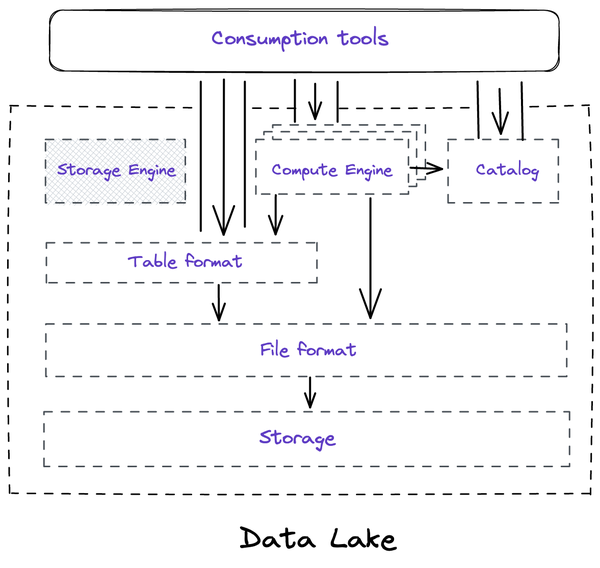
\includegraphics[width=\textwidth,height=.75\textheight,keepaspectratio]{./Figures/chapter-04/datalake_table_format}};
            % Place text and arrow
            \draw[<-, thick] (image) -- ++(4,1) node[right, align=left,font=\small, text=gray] {Apache Iceberg: The Definitive Guide: \\Data Lakehouse Functionality,\\ Performance, and Scalability\\ on the Data Lake\\ PUBLISHED BY:
            O'Reilly Media, Inc.};
        \end{tikzpicture}
        \captionof{figure}{Technical components in a data lake}
    \end{minipage}
\end{frame}

%%%%%%%%%%%%%%%%%%%%%%%%%%%%%%%%%%%%%%%%%%%%%%%%%%%%%%
\begin{frame}{Technical components in a data lake}
    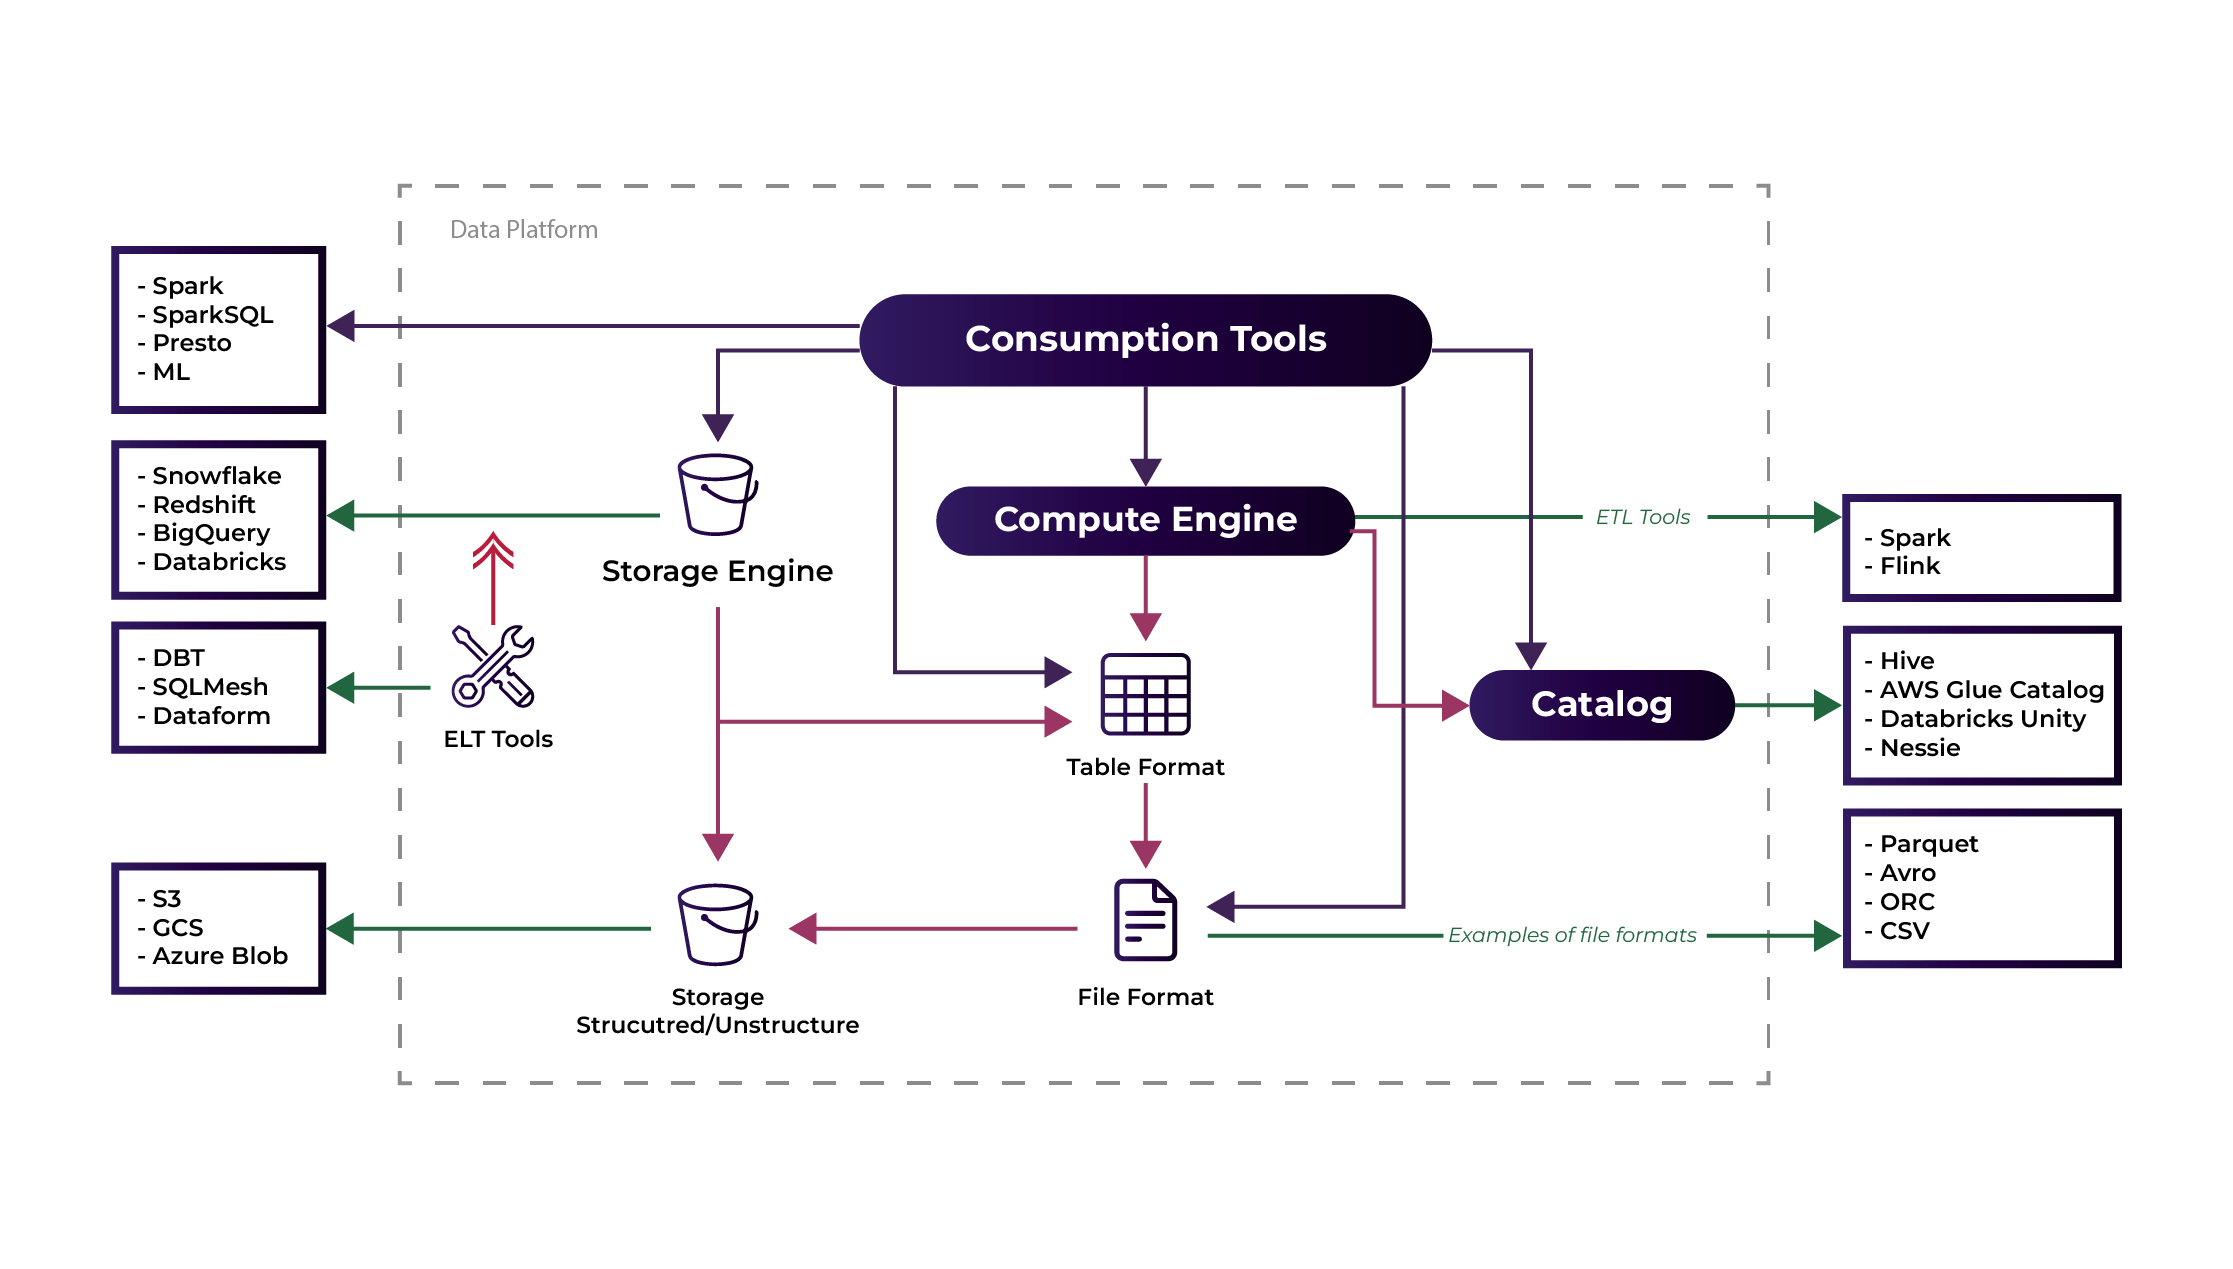
\includegraphics[width=\textwidth,height=.8\textheight,keepaspectratio]{./Figures/chapter-04/DataPlatform};
\end{frame}
%%%%%%%%%%%%%%%%%%%%%%%%%%%%%%%%%%%%%%%%%%%%%%%%%%%%%%
%Ch.04-06   | Running Spark

\subsection{Running Spark}\label{subsec:running-spark}
\begin{frame}
    \frametitle{Running Spark for Beginners}

    \begin{itemize}
        \item \textbf{Databricks Community Edition:} The simplest option for Spark beginners. A free version that's easy to use for learning and small projects.
        \item \textbf{Install Spark Locally:} For hands-on experience with Spark's core features on your own machine.
        \item \textbf{Spark on Docker:} For a flexible, containerized environment that can replicate a production setup.
    \end{itemize}

    \bigskip % Adds a bit more vertical space

    \emph{Note:} For those new to Spark, starting with the Databricks Community Edition is highly recommended due to its user-friendly interface and comprehensive documentation.

\end{frame}
\begin{frame}
    \centering
    \vfill
    \Large{Demo: Databricks Community Edition!}
    \vfill
\end{frame}

\begin{frame}
    \centering
    \vfill
    \Large{Demo: Install Spark Locally on Mac!}
    \vfill
\end{frame}

\begin{frame}
    \centering
    \vfill
    \Large{Demo: Install Spark Locally on Windows!}
    \vfill
\end{frame}

\begin{frame}
    \centering
    \vfill
    \Large{Demo: Install Spark Locally on Linux!}
    \vfill
\end{frame}

\begin{frame}
    \centering
    \vfill
    \Large{Demo: Spark Shell!}
    \vfill
\end{frame}

\begin{frame}
    \centering
    \vfill
    \Large{Demo: Spark SQL!}
    \vfill
\end{frame}
%%%%%%%%%%%%%%%%%%%%%%%%%%%%%%%%%%%%%%%%%%%%%%%%%%%%%%
%Ch.04-11   | From Map Reduce To Spark

\subsection{From MapReduce to Apache Spark}\label{subsec:from-mapreduce-to-apache-spark}

%%%%%%%%%%%%%%%%%%%%%%%%%%%%%%%%%%%%%%%%%%%%%%%%%%%%%%
\begin{frame}
    \frametitle{The basic idea of MapReduce}
    \begin{itemize}
        [<+->]
        \item Assume we need to launch a high-throughput bulk-production sandwich shop.
        \item This sandwich has a lot of raw ingredients, and our target is to produce the sandwich as quickly as possible.
        \item To make the production very quickly we need to distribute the tasks between the  \textcolor{orange}{\textit{workers}}.
    \end{itemize}
    \footnotetext[1]{This example taken from  \href{https://reberhardt.com/cs110/summer-2018/lecture-notes/lecture-14/}{https://reberhardt.com/cs110/summer-2018/lecture-notes/lecture-14/}    }
\end{frame}
%%%%%%%%%%%%%%%%%%%%%%%%%%%%%%%%%%%%%%%%%%%%%%%%%%%%%%
\begin{frame}
    \frametitle{The basic idea of MapReduce}
    We break this into three stages
    \begin{itemize}
        [<+->]
        \item Map.
        \item Shuffle/Group (Mapper Intermediates).
        \item Reduce
    \end{itemize}
    \footnotetext[1]{This example taken from  \href{https://reberhardt.com/cs110/summer-2018/lecture-notes/lecture-14/}{https://reberhardt.com/cs110/summer-2018/lecture-notes/lecture-14/}    }
\end{frame}
%%%%%%%%%%%%%%%%%%%%%%%%%%%%%%%%%%%%%%%%%%%%%%%%%%%%%%
\begin{frame}
    \frametitle{Map}
    We distribute our raw ingredients amongst the workers.
    \begin{figure}
        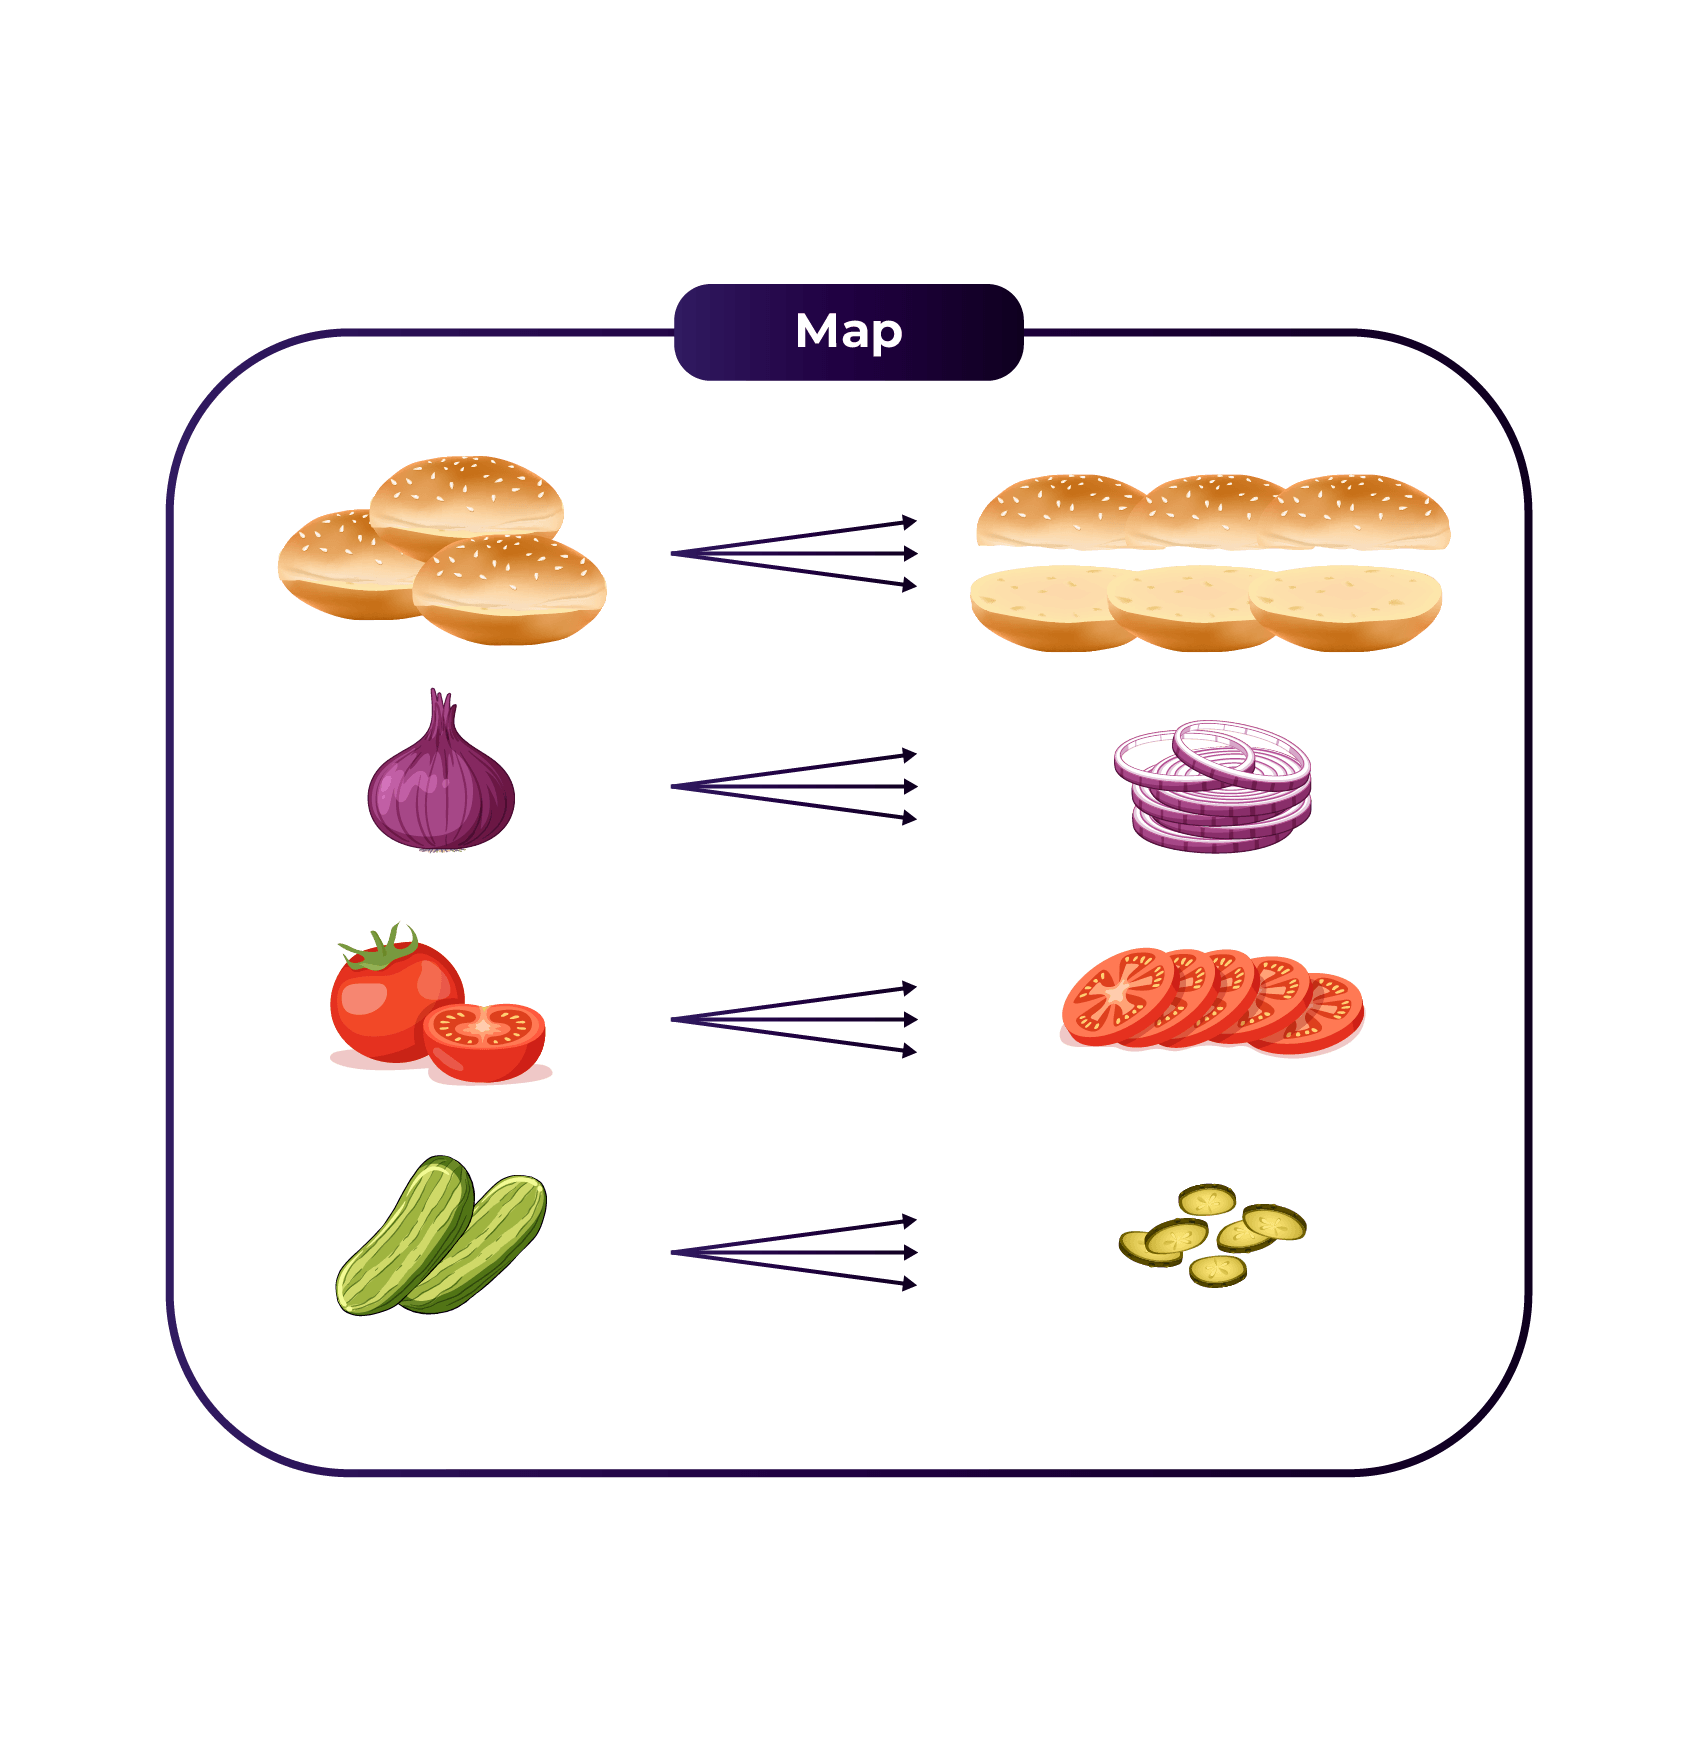
\includegraphics[width=.5\textwidth,height=.8\textheight]{./Figures/chapter-04/map}\label{fig:map}
    \end{figure}
    \footnotetext[1]{{\tiny This example taken from  \href{https://reberhardt.com/cs110/summer-2018/lecture-notes/lecture-14/}{https://reberhardt.com/cs110/summer-2018/lecture-notes/lecture-14/}    } }
\end{frame}
%%%%%%%%%%%%%%%%%%%%%%%%%%%%%%%%%%%%%%%%%%%%%%%%%%%%%%
\begin{frame}
    \frametitle{Shuffle/Group}
    We will organise and group the processed ingredients into piles, so that making a sandwich becomes easy.
    \begin{figure}
        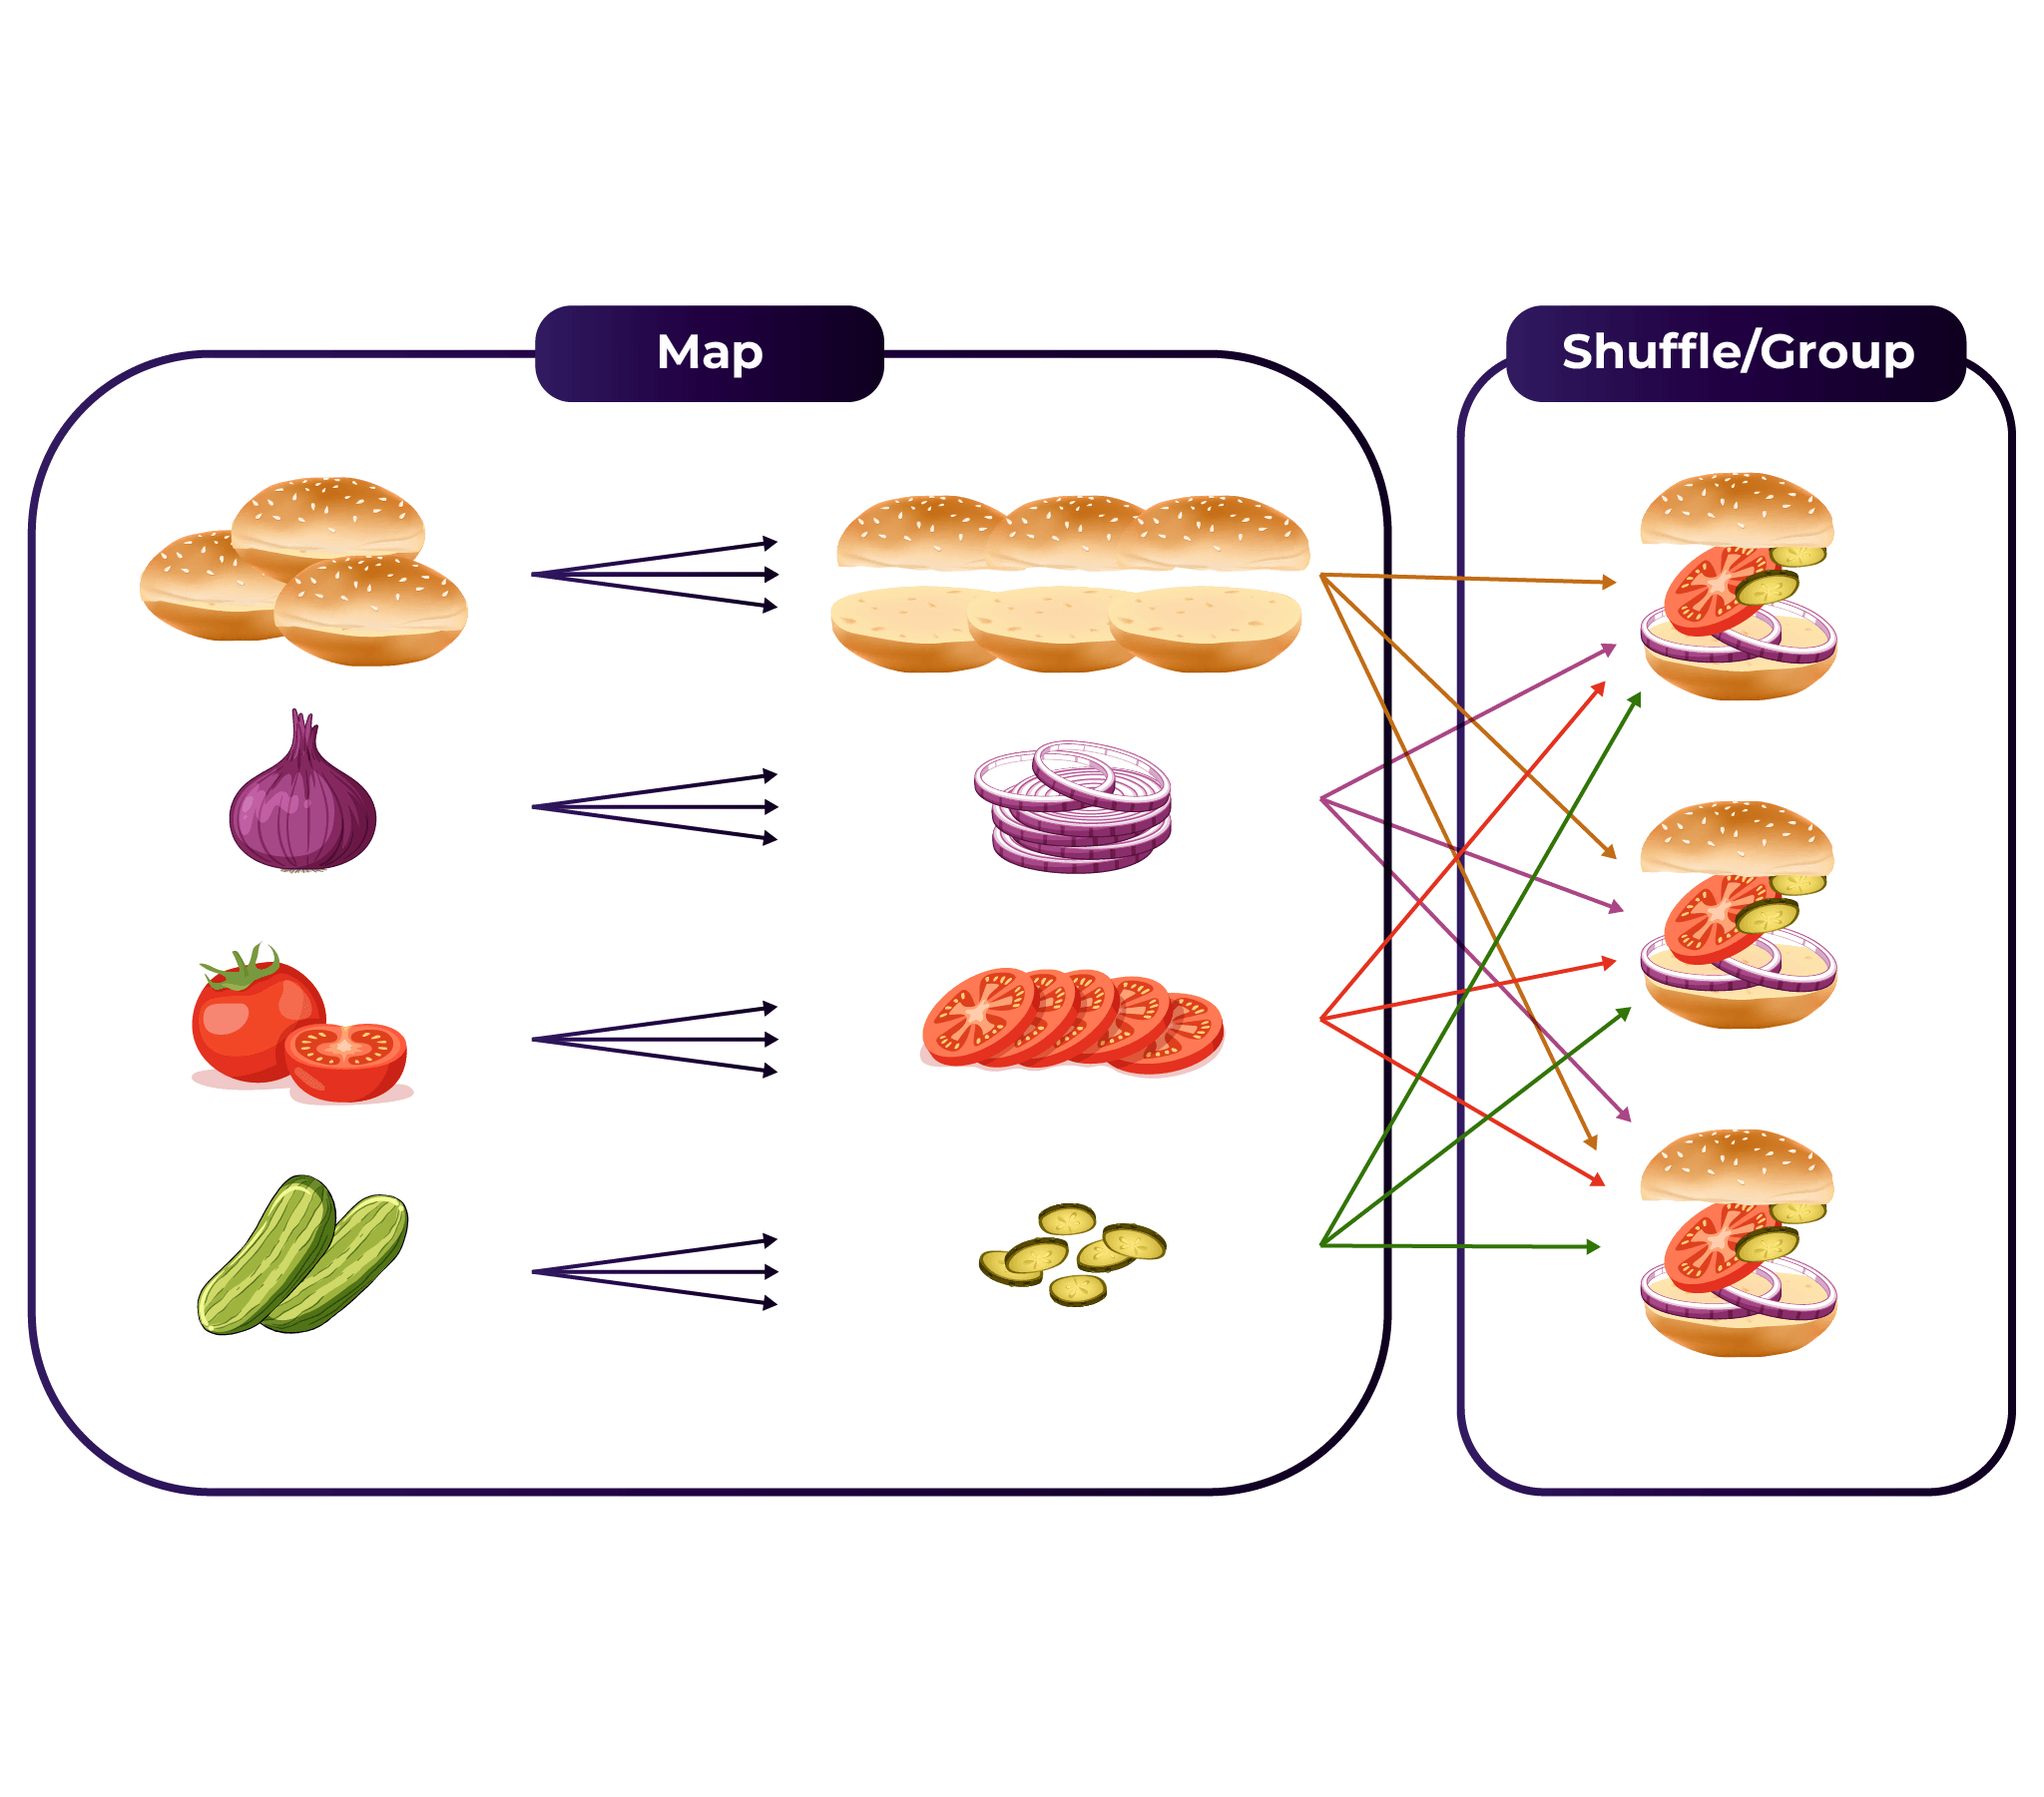
\includegraphics[width=.7\textwidth,height=.8\textheight]{./Figures/chapter-04/map_shuffle}\label{fig:map_shuffle}
    \end{figure}
    \footnotetext[1]{{\tiny This example taken from  \href{https://reberhardt.com/cs110/summer-2018/lecture-notes/lecture-14/}{https://reberhardt.com/cs110/summer-2018/lecture-notes/lecture-14/}    }}
\end{frame}
%%%%%%%%%%%%%%%%%%%%%%%%%%%%%%%%%%%%%%%%%%%%%%%%%%%%%%
\begin{frame}
    \frametitle{Reduce}
    we’ll combine the ingredients into a sandwich
    \begin{figure}
        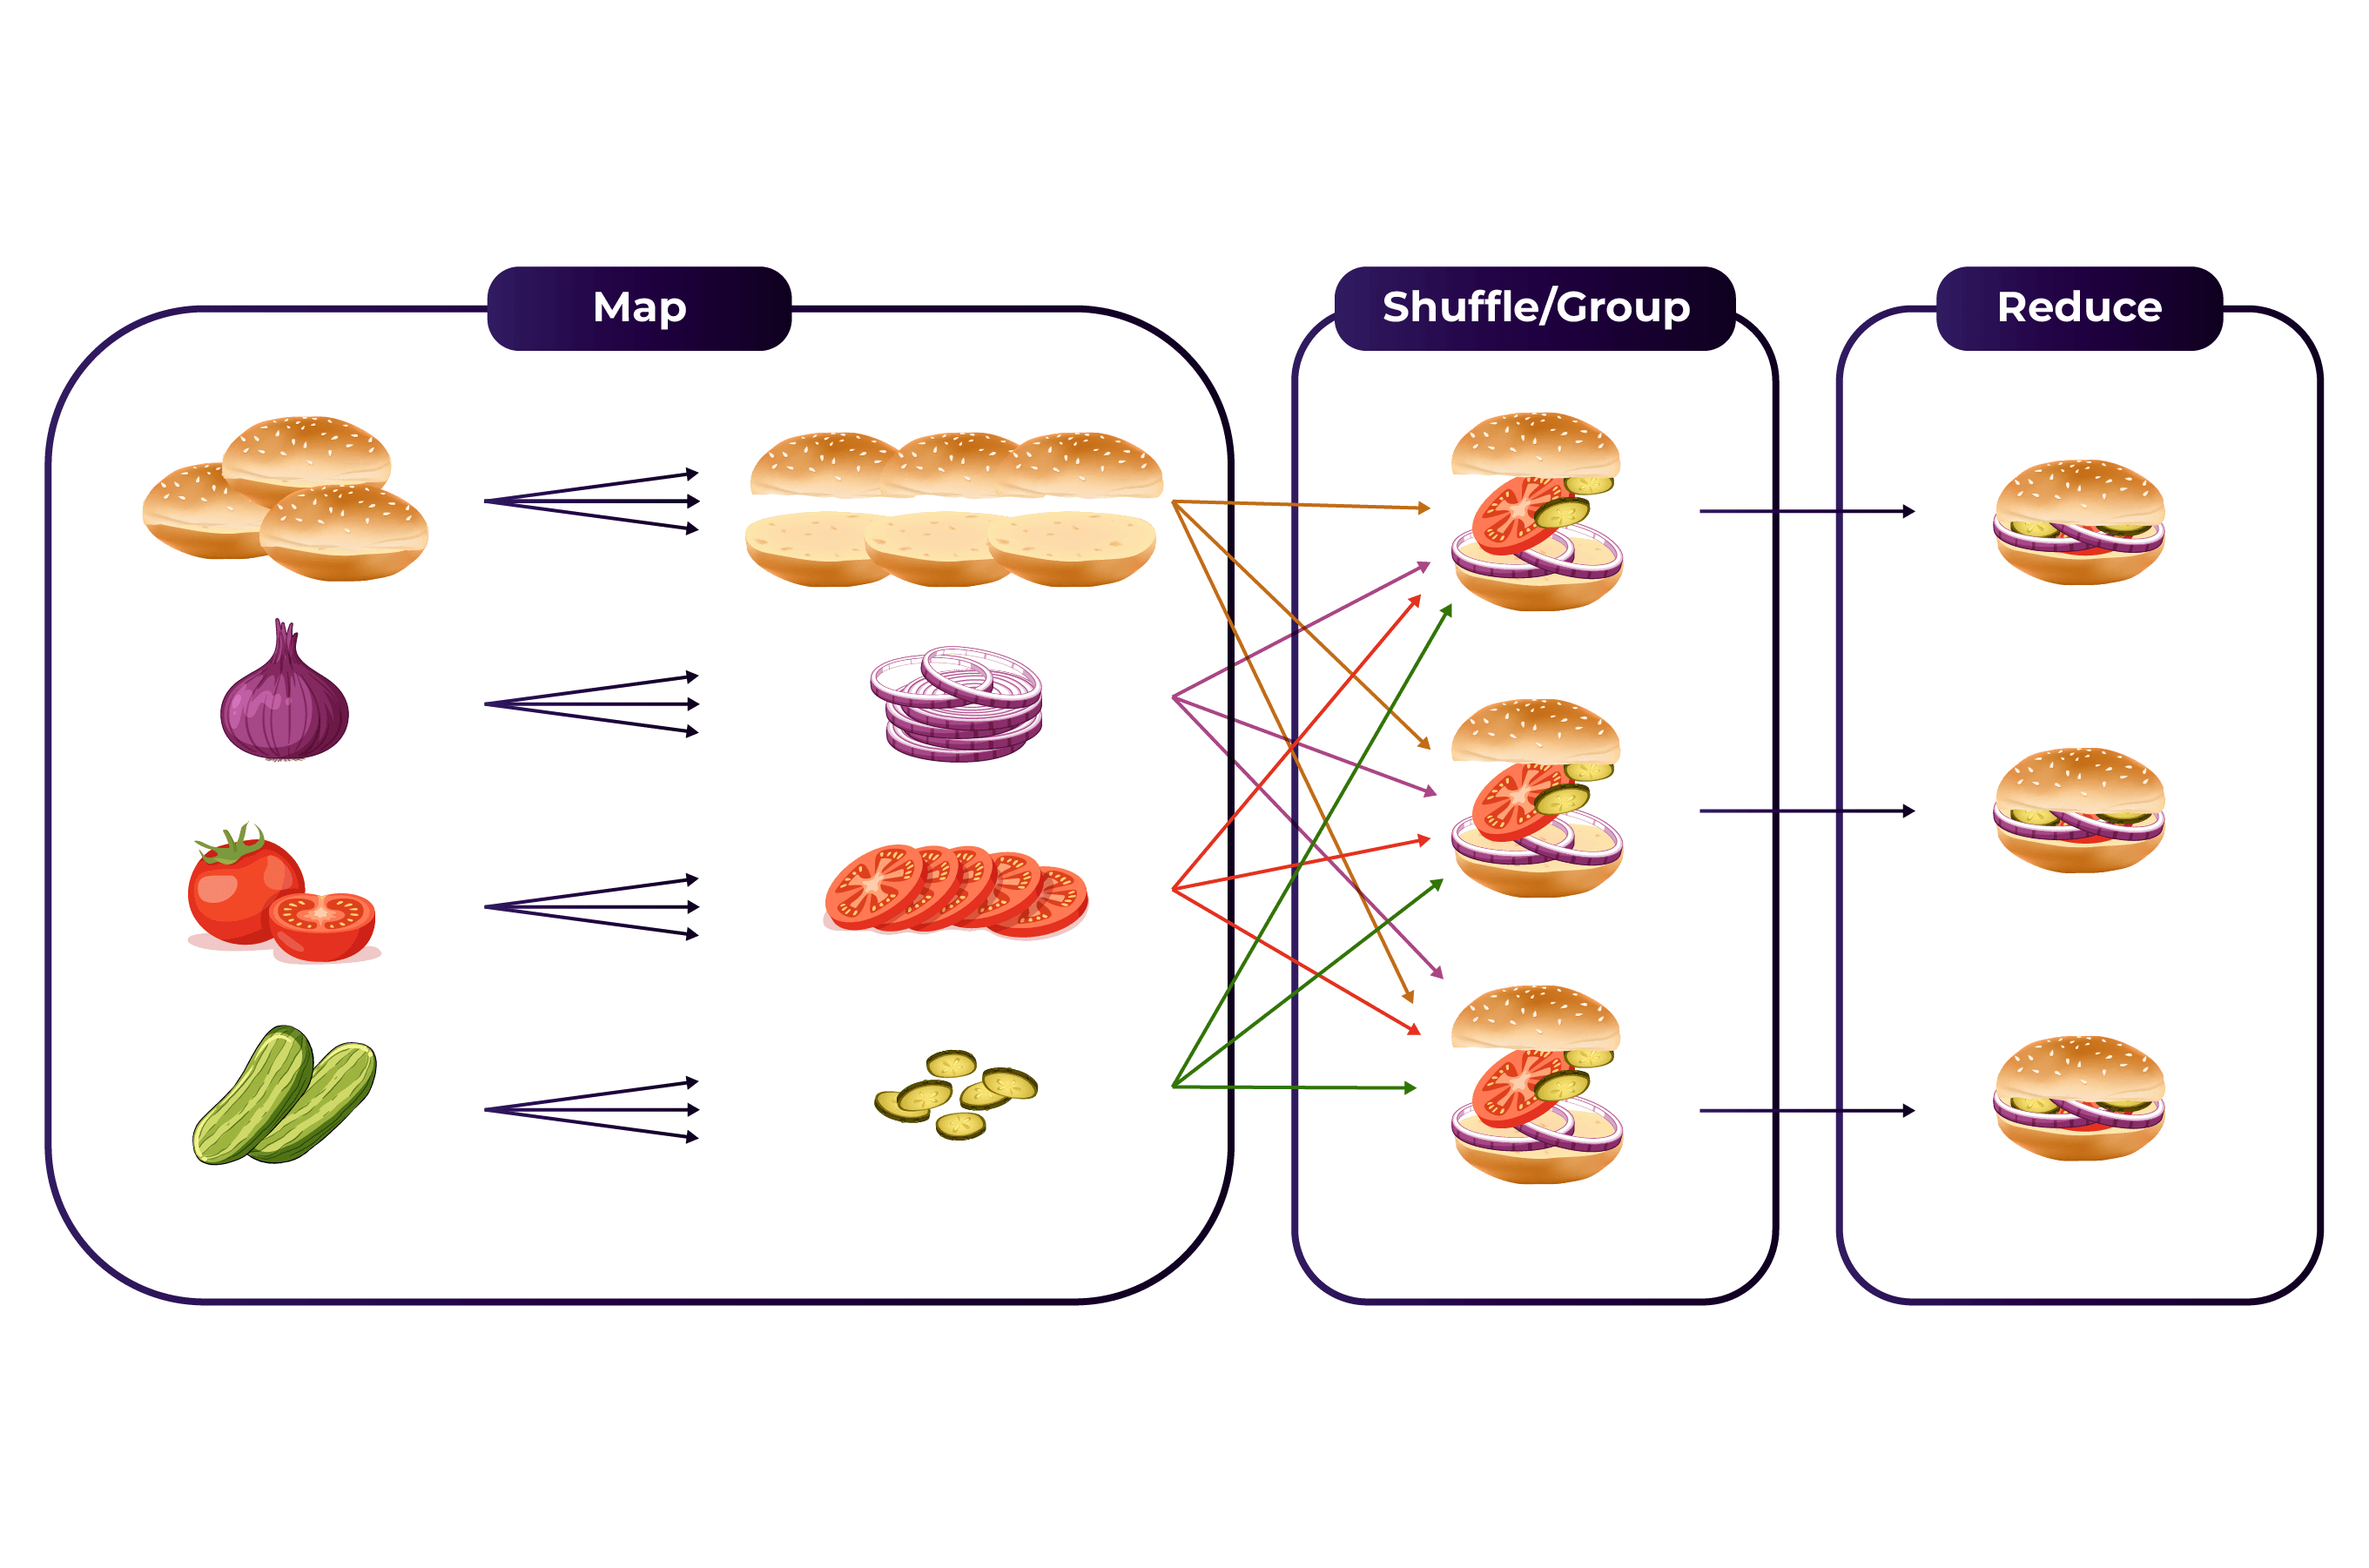
\includegraphics[width=.96\textwidth,height=.6\textheight]{./Figures/chapter-04/map_reduce}\label{fig:map_reduce}
    \end{figure}
    \footnotetext[1]{ {\tiny This example taken from  \href{https://reberhardt.com/cs110/summer-2018/lecture-notes/lecture-14/}{https://reberhardt.com/cs110/summer-2018/lecture-notes/lecture-14/}    }}
\end{frame}
%%%%%%%%%%%%%%%%%%%%%%%%%%%%%%%%%%%%%%%%%%%%%%%%%%%%%%
\begin{frame}
    \frametitle{Map Reduce Bottelneck}
    \begin{figure}
        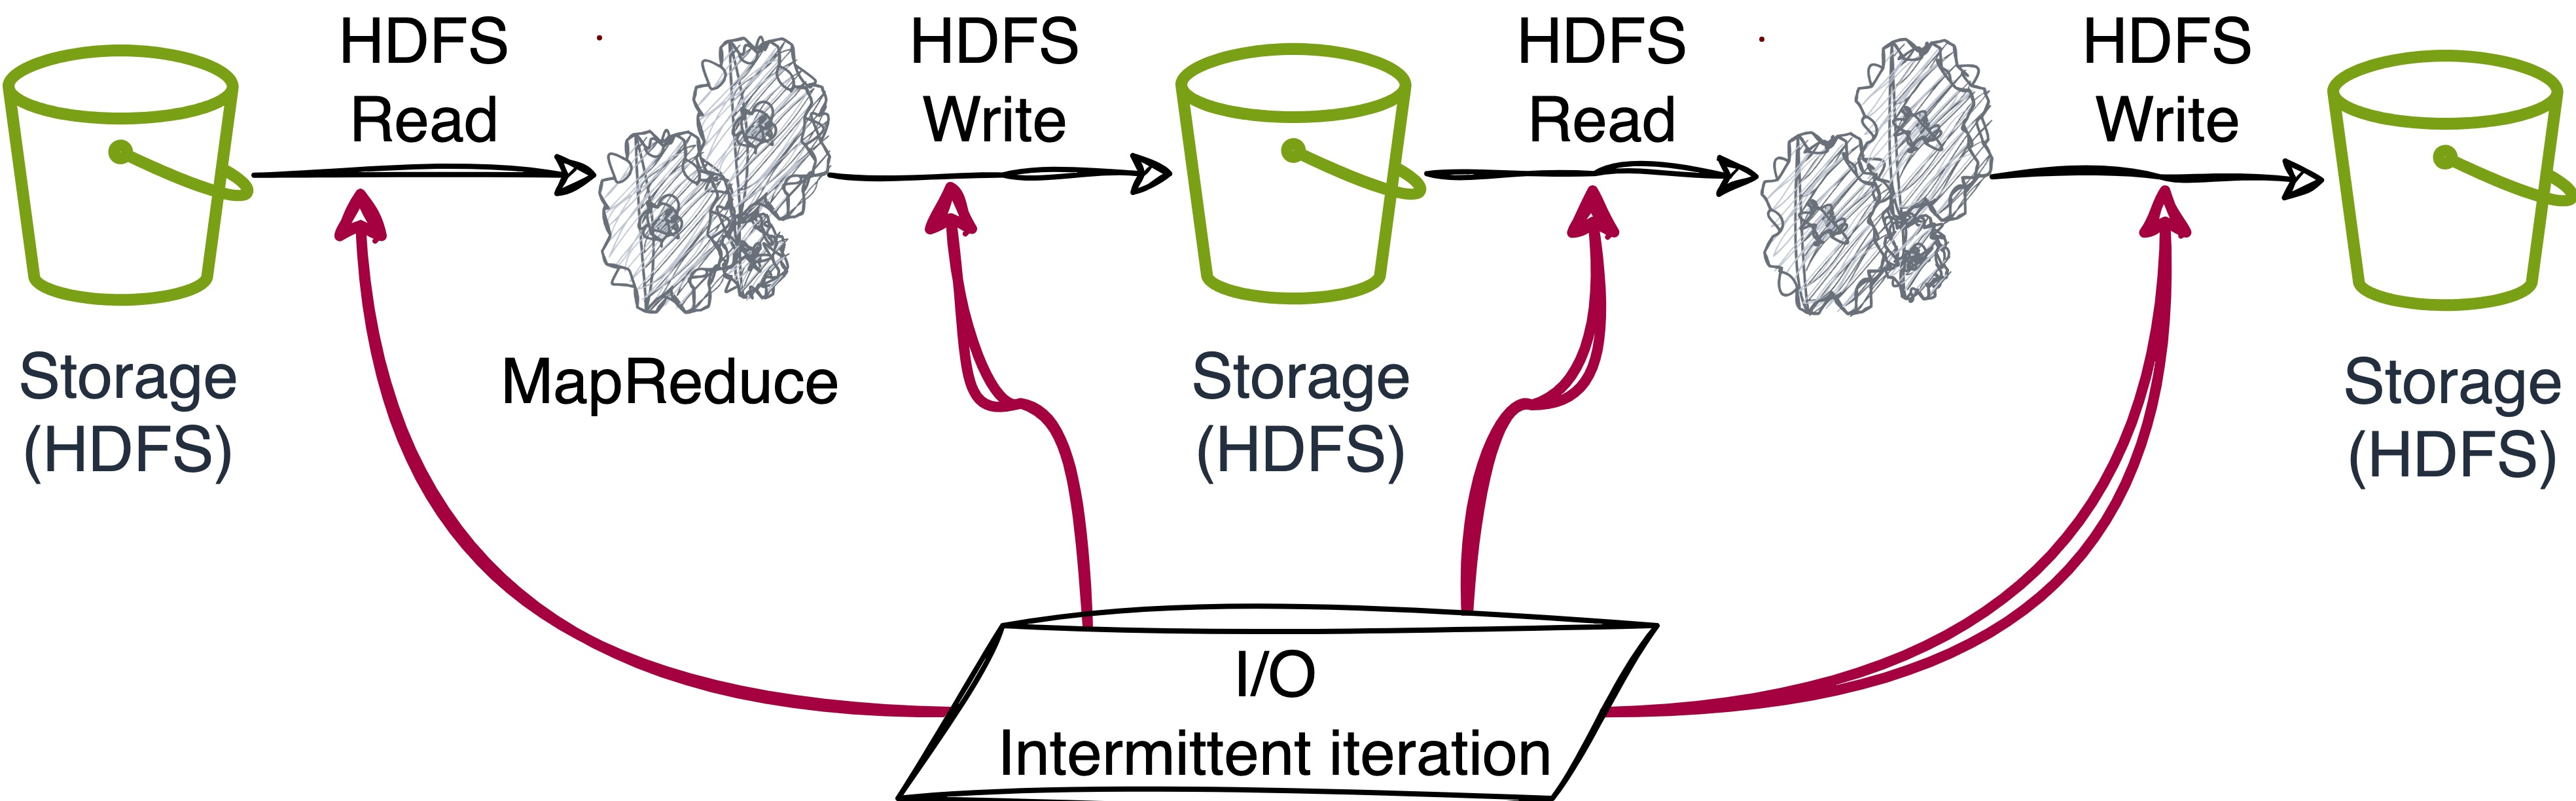
\includegraphics[width=.96\textwidth,height=.6\textheight]{./Figures/chapter-04/MR}\label{fig:figure4}
    \end{figure}
\end{frame}
%%%%%%%%%%%%%%%%%%%%%%%%%%%%%%%%%%%%%%%%%%%%%%%%%%%%%%
\begin{frame}
    \frametitle{Spark Motivation}
    \begin{itemize}

        \item In-Memory Processing.

        \item Resilient Distributed Datasets (RDDs).%**: Spark uses RDDs to perform parallel operations on data stored across cluster nodes, minimizing disk I/O by keeping data in RAM.

        \item Optimized Execution (DAG execution engine).%: The DAG execution engine organizes computations efficiently, reducing unnecessary operations and combining tasks to lower data movement.

        \item Caching.%: Spark allows for the caching of intermediate data in memory, benefiting iterative algorithms that reuse data, thereby avoiding repetitive disk access.

        \item Advanced Optimization (Catalyst optimizer and Tungsten).%: With components like the Catalyst optimizer and Tungsten for memory and CPU efficiency, Spark streamlines execution, making it ideal for fast, iterative processing over big data.

    \end{itemize}
\end{frame}
%%%%%%%%%%%%%%%%%%%%%%%%%%%%%%%%%%%%%%%%%%%%%%%%%%%%%%
% Ch.04-12   | Spark Characteristics

\subsection{Spark Characteristics}\label{subsec:characteristics-apache-spark}

\begin{frame}
    \frametitle{Spark Characteristics}
    \begin{itemize}
        \item Speed.
        \item Ease of use.
        \item Modularity.
        \item Extensibility.
    \end{itemize}
\end{frame}


\begin{frame}
    \frametitle{Spark Characteristics: Speed}
    \begin{itemize}
        \item Spark's speed is achieved through various strategies.
        \begin{itemize}
            \item \textbf{Hardware Utilization:} Spark leverages commodity hardware with extensive memory and multiple cores, utilizing efficient multithreading and parallel processing for improved performance.
            \item \textbf{Directed Acyclic Graph (DAG):} Spark constructs computations as a DAG. Its scheduler and optimizer create an efficient graph, allowing parallel task execution across cluster workers. \textit{\color{blue}This topic will be discussed later.}
            %TODO: about Spark DAG scheduler
        \end{itemize}
    \end{itemize}

\end{frame}

\begin{frame}
    \frametitle{Spark Characteristics: Speed}
    \begin{itemize}
        \item Spark's speed is achieved through various strategies.
        \begin{itemize}
            \item \textbf{Tungsten Execution Engine:} Tungsten enhances Spark's speed by optimizing memory management,
            shifting from JVM-managed objects to direct binary processing, and employing cache-optimized algorithms and advanced code generation. These improvements reduce CPU and memory bottlenecks, significantly boosting performance. \textit{\color{blue}This topic will be discussed later.}
        \end{itemize}
    \end{itemize}

\end{frame}

\begin{frame}
    \frametitle{Spark Characteristics: Ease of use}
    \begin{itemize}
        \item Spark simplifies big data processing with an abstraction called a Resilient Distributed Dataset (RDD).
        \item RDDs serve as the foundation for higher-level data structures like DataFrames and Datasets in Spark. \textit{\color{blue}This topic will be discussed later.}
        \item Compared with MapReduce and other complex distributed processing frameworks, Spark provides a simple programming model with a range of transformations and actions.
    \end{itemize}
\end{frame}


\begin{frame}
    \frametitle{Spark Characteristics: Modularity}
    \begin{itemize}
        \item Spark operations are flexible, supporting various workloads and languages: Scala, Java, Python, SQL, and R.
        \item It provides unified libraries with comprehensive APIs (SparkSQL, Structured Streaming, MLlib, and GraphX).
        \item These modules allow Spark to handle different workloads under a single engine.
        \item With Spark, you can develop a single application for diverse tasks without the need for separate engines or learning different APIs, achieving a unified processing framework.
    \end{itemize}
\end{frame}

\begin{frame}
    \frametitle{Spark Characteristics: Extensibility}
    \begin{itemize}
        \item Spark focuses on its fast, parallel computation engine rather than on storage (Unlike Apache Hadoop, which included both storage and compute).
    \end{itemize}
\end{frame}


\begin{frame}
    \frametitle{Spark Characteristics: Extensibility}
    \begin{itemize}
        \item Spark can process data from various sources like Hadoop, Cassandra, HBase, MongoDB, Hive, RDBMSs, and others in memory for faster processing.
        \item Spark's \texttt{DataFrameReader}s and \texttt{DataFrameWriter}s allow Spark to interact with even more data sources, such as Kafka, Kinesis, Azure Storage, and Amazon S3.
        \item The Spark community maintains a list of third-party packages, enhancing its ecosystem with connectors for external data sources, performance monitors, and more.
    \end{itemize}
\end{frame}
